\chapter{Modelagem Matemática e Geração Simbólica}
\label{cap:modelagem}

Este capítulo apresenta, em detalhe, a arquitetura de modelagem matemática implementada no núcleo computacional do \textit{Hephaestus}. O objetivo central é descrever como a cadeia cinemática de um manipulador genérico de $N$ graus de liberdade , em ambiente terrestre ou subaquático , é traduzida em expressões simbólicas fechadas para a matriz de inércia $M(q)$, o vetor de Coriolis $C(q,\dot{q})$ e o vetor de gradiente de potencial $G(q)$, bem como o processo de compilação dessas expressões em funções numéricas otimizadas para simulação em tempo real. A exposição combina a fundamentação teórica dos conceitos revisados no Capítulo~\ref{cap:revisao} com as escolhas concretas de implementação que diferenciam o \textit{Hephaestus} das abordagens clássicas.

% ==============================================================================
\section{Visão Geral da Arquitetura}
% ==============================================================================

A \textit{engine} matemática do \textit{Hephaestus} é organizada em uma hierarquia de classes: \texttt{RobotMathEngine} , responsável pela modelagem em ambiente seco (ar) , e \texttt{RobotMathHydro} , subclasse que estende o modelo para ambiente subaquático, incorporando os efeitos de massa adicionada e empuxo. A filosofia de projeto segue o princípio de separação entre a camada simbólica (geração das equações exatas) e a camada numérica (avaliação eficiente em tempo de simulação), conforme proposto por Meurer et al. \cite{meurer2017sympy}.

O fluxo completo de processamento é organizado em quatro etapas sequenciais, refletidas nos métodos públicos da classe:

\begin{enumerate}
    \item \textbf{Cinemática Simbólica} (\texttt{step\_1\_kinematics}): construção das transformações homogêneas acumuladas, das posições dos centros de massa e das velocidades angulares de cada elo.
    \item \textbf{Matriz de Inércia e Gradiente de Potencial} (\texttt{step\_2\_jacobian\_M\_G}): derivação simbólica de $M(q)$ e $G(q)$ por meio do método do Jacobiano da inércia, com rotação explícita dos tensores locais para o referencial global.
    \item \textbf{Vetor de Coriolis} (\texttt{step\_3\_coriolis\_combined}): cálculo dos símbolos de Christoffel de segunda espécie a partir de $\partial M/\partial q_k$, com suporte a paralelismo por múltiplos processos.
    \item \textbf{Preparação e Exportação} (\texttt{step\_4\_prepare\_export}): substituição de símbolos dinâmicos por variáveis estáticas e empacotamento do modelo para o módulo de simulação.
\end{enumerate}

Essa organização modular permite que o usuário inspecione o estado intermediário após cada etapa, facilitando a depuração matemática e a validação pedagógica das equações geradas , objetivo central de uma plataforma didática de código aberto \cite{corke2021toolbox}.

% ==============================================================================
\section{Representação da Cadeia Cinemática}
% ==============================================================================

\subsection{Configuração de Juntas e Máscara de Vetores de Elo}

A cadeia cinemática é especificada pelo usuário por meio de dois parâmetros de entrada:

\begin{itemize}
    \item \texttt{joint\_config}: lista de strings descrevendo o tipo e eixo de cada junta. O primeiro caractere indica o tipo , \texttt{'R'} para junta de revolução (\textit{Revolute}) ou \texttt{'D'} para junta prismática (\textit{Displacement}) , e o segundo caractere indica o eixo de movimento (\texttt{'x'}, \texttt{'y'} ou \texttt{'z'}).
    \item \texttt{link\_vectors\_mask}: lista de vetores tridimensionais $(u_x, u_y, u_z)$ que definem a direção do elo estrutural ligado à respectiva junta no referencial local. O comprimento efetivo do elo é parametrizado pelo símbolo escalar $L_i$, de modo que o vetor de translação do elo $i$ é $\vec{r}_i = (u_x, u_y, u_z)^i \cdot L_i$.
\end{itemize}

Essa parametrização admite qualquer topologia de cadeia serial aberta, incluindo configurações com juntas prismáticas mistas , fundamentais para modelar o grau de liberdade de afundamento de veículos subaquáticos , e configurações com elos de comprimento nulo (vetor máscara zero), usadas para modelar as três rotações do veículo base de um UVMS sem translação associada \cite{antonelli2014modelling, fossen2011handbook}.

A escolha de uma parametrização matricial de rotações diretas em vez da convenção de Denavit-Hartenberg (DH) \cite{denavit1955kinematic} foi deliberada. Embora a convenção DH seja amplamente ensinada \cite{craig1989introduction, spong2020robot}, ela impõe restrições geométricas sobre o posicionamento dos eixos de coordenadas que dificultam a representação de certas arquiteturas (e.g., juntas com deslocamentos paralelos). A representação por matrizes de rotação elementares por eixo-ângulo, adotada no \textit{Hephaestus}, é algebricamente transparente e diretamente integrável com o módulo de mecânica simbólica do SymPy \cite{meurer2017sympy, leu1986automated}.

\subsection{Símbolos Dinâmicos e Parâmetros}

Para cada junta $i$, são criados automaticamente os seguintes símbolos SymPy:

\begin{itemize}
    \item $q_i(t)$, $\dot{q}_i(t)$: variáveis de junta e sua derivada temporal, instanciadas como \texttt{dynamicsymbols} para suportar diferenciação automática \cite{meurer2017sympy};
    \item $m_i$, $L_i$: massa e comprimento do elo $i$;
    \item $cx_i$, $cy_i$, $cz_i$: coordenadas do centro de massa no referencial local do elo $i$;
    \item $Ixx_i$, $Iyy_i$, $Izz_i$: momentos principais de inércia no referencial local.
\end{itemize}

Adicionalmente, o símbolo escalar $g$ representa a aceleração gravitacional. No modo hidrodinâmico, o símbolo $\rho$ (densidade do fluido) e os volumes deslocados $\text{vol}_i$ são adicionados à lista de parâmetros. Todos esses símbolos são agrupados em \texttt{params\_list}, que serve como assinatura da função compilada \cite{meurer2017sympy}. Essa abordagem garante que as equações geradas sejam \emph{parametricamente completas}: um único modelo simbólico serve para qualquer instância paramétrica do robô, sem necessidade de recomputação quando os valores físicos são alterados , propriedade ausente em geradores de código que utilizam substituição numérica direta \cite{hollerbach1980recursive}.

% ==============================================================================
\section{Cinemática Simbólica Direta}
\label{sec:cinematica_simbolica}
% ==============================================================================

\subsection{Transformações Homogêneas Acumuladas}

A cinemática direta é construída iterativamente sobre a cadeia de elos. Para a junta $i$ do tipo revolução em torno do eixo $\hat{a}_i$ (expresso no referencial global acumulado $R_{\text{acc}}$), a matriz de rotação local é:
\begin{equation}
    R_j^{(i)} = \exp\!\left(\hat{a}_i^{(l)}\,q_i\right), \quad \hat{a}_i^{(l)} \in \{\hat{x}, \hat{y}, \hat{z}\},
    \label{eq:rot_local}
\end{equation}
onde:
\begin{itemize}
    \item $R_j^{(i)} \in \mathbb{R}^{3\times 3}$ é a matriz de rotação local introduzida pela junta $i$;
    \item $\hat{a}_i^{(l)}$ é o eixo unitário de rotação da junta no referencial local, mapeado para as matrizes elementares $R_x$, $R_y$ ou $R_z$ conforme o caractere do tipo de junta;
    \item $q_i$ é a coordenada generalizada (ângulo de rotação) da junta $i$;
    \item $\exp(\cdot)$ denota a exponencial matricial, equivalente à fórmula de Rodrigues para rotações elementares \cite{craig1989introduction, siciliano2009robotics}.
\end{itemize}

Para a junta prismática ao longo do eixo $\hat{a}_i^{(l)}$:
\begin{equation}
    R_j^{(i)} = I_3, \quad P_j^{(i)} = \hat{a}_i^{(l)}\, q_i.
    \label{eq:prism_local}
\end{equation}
onde:
\begin{itemize}
    \item $R_j^{(i)} = I_3$ é a matriz identidade $3\times 3$, indicando que a junta prismática não introduz rotação local;
    \item $P_j^{(i)} \in \mathbb{R}^{3}$ é o vetor de translação devido ao deslocamento da junta;
    \item $\hat{a}_i^{(l)}$ é o eixo unitário de translação da junta no referencial local;
    \item $q_i$ é a coordenada generalizada (deslocamento linear) da junta $i$.
\end{itemize}

A transformação homogênea $4 \times 4$ acumulada até o extremo do elo $i$ é:
\begin{equation}
    T_i = T_{i-1} \cdot T_{\text{junta},i} \cdot T_{\text{elo},i},
    \label{eq:T_acumulada}
\end{equation}
onde:
\begin{itemize}
    \item $T_i \in \mathbb{R}^{4\times 4}$ é a transformação homogênea acumulada do referencial global até o extremo do elo $i$;
    \item $T_{i-1}$ é a transformação acumulada do elo anterior, com $T_0 = I_4$ (identidade $4\times 4$);
    \item $T_{\text{junta},i}$ encapsula a rotação/translação introduzida pela junta $i$ (Equações~\eqref{eq:rot_local} ou~\eqref{eq:prism_local});
    \item $T_{\text{elo},i}$ codifica a translação estrutural do elo, com vetor $\vec{r}_i = L_i \cdot \texttt{link\_vectors\_mask}[i]$;
    \item $L_i$ é o comprimento simbólico do elo $i$.
\end{itemize}
Isso é computado simbolicamente pelo SymPy, produzindo expressões fechadas que dependem de $\{q_1, \ldots, q_N\}$ e $\{L_1, \ldots, L_N\}$ \cite{spong2020robot}.

\subsection{Posições dos Centros de Massa no Referencial Global}

A posição global do centro de massa do elo $i$ é obtida por:
\begin{equation}
    \vec{p}_{\text{cm},i} = T_{\text{at-joint},i} \cdot \begin{bmatrix} cx_i \\ cy_i \\ cz_i \\ 1 \end{bmatrix}_{\!(1:3)},
    \label{eq:pcm_global}
\end{equation}
onde:
\begin{itemize}
    \item $\vec{p}_{\text{cm},i} \in \mathbb{R}^{3}$ é a posição do centro de massa do elo $i$ no referencial global;
    \item $T_{\text{at-joint},i} = T_{i-1} \cdot T_{\text{junta},i}$ é a transformação homogênea até o \emph{início} do elo $i$ (antes da translação estrutural);
    \item $[cx_i,\, cy_i,\, cz_i]$ são as coordenadas do centro de massa no referencial local do elo $i$;
    \item o índice $(1:3)$ indica a extração das três primeiras componentes do vetor homogêneo resultante.
\end{itemize}
Essa convenção separa o CM do extremo do elo, permitindo modelar distribuições de massa arbitrárias ao longo do elo sem hipóteses simplificadoras de CM centrado \cite{siciliano2009robotics, spong2020robot}.

\subsection{Velocidades Angulares Simbólicas}

A velocidade angular global do elo $i$ é acumulada recursivamente:
\begin{equation}
    \vec{\omega}_i = \vec{\omega}_{i-1} + R_{\text{acc},i-1} \cdot \hat{a}_i^{(l)} \cdot \dot{q}_i \quad \text{(juntas R)}, \qquad
    \vec{\omega}_i = \vec{\omega}_{i-1} \quad \text{(juntas D)}.
    \label{eq:omega_rec}
\end{equation}
onde:
\begin{itemize}
    \item $\vec{\omega}_i \in \mathbb{R}^{3}$ é a velocidade angular do elo $i$ expressa no referencial global;
    \item $\vec{\omega}_{i-1}$ é a velocidade angular do elo anterior na cadeia, com $\vec{\omega}_0 = \vec{0}$;
    \item $R_{\text{acc},i-1} \in \mathbb{R}^{3\times 3}$ é a matriz de rotação global acumulada até o elo $i-1$;
    \item $\hat{a}_i^{(l)}$ é o eixo unitário de rotação da junta $i$ no referencial local;
    \item $\dot{q}_i$ é a velocidade generalizada (taxa angular) da junta $i$;
    \item ``juntas R'' refere-se a juntas rotacionais e ``juntas D'' a juntas prismáticas (\textit{Displacement}), que não contribuem para a velocidade angular.
\end{itemize}

Essa recorrência segue a formulação vetorial da velocidade angular para cadeias seriais \cite{craig1989introduction, luh1980online}. O resultado é uma expressão simbólica linear em $\{\dot{q}_1, \ldots, \dot{q}_N\}$, cuja derivada em relação a $\dot{q}_j$ fornece diretamente a $j$-ésima coluna do Jacobiano angular $J_{\omega,i}$ \cite{siciliano2009robotics}. O fluxo completo da etapa de cinemática simbólica , da especificação de juntas ao Jacobiano geométrico , é sintetizado na Figura~\ref{fig:cinem_simbolica}.

\begin{figure}[htbp]
    \centering
    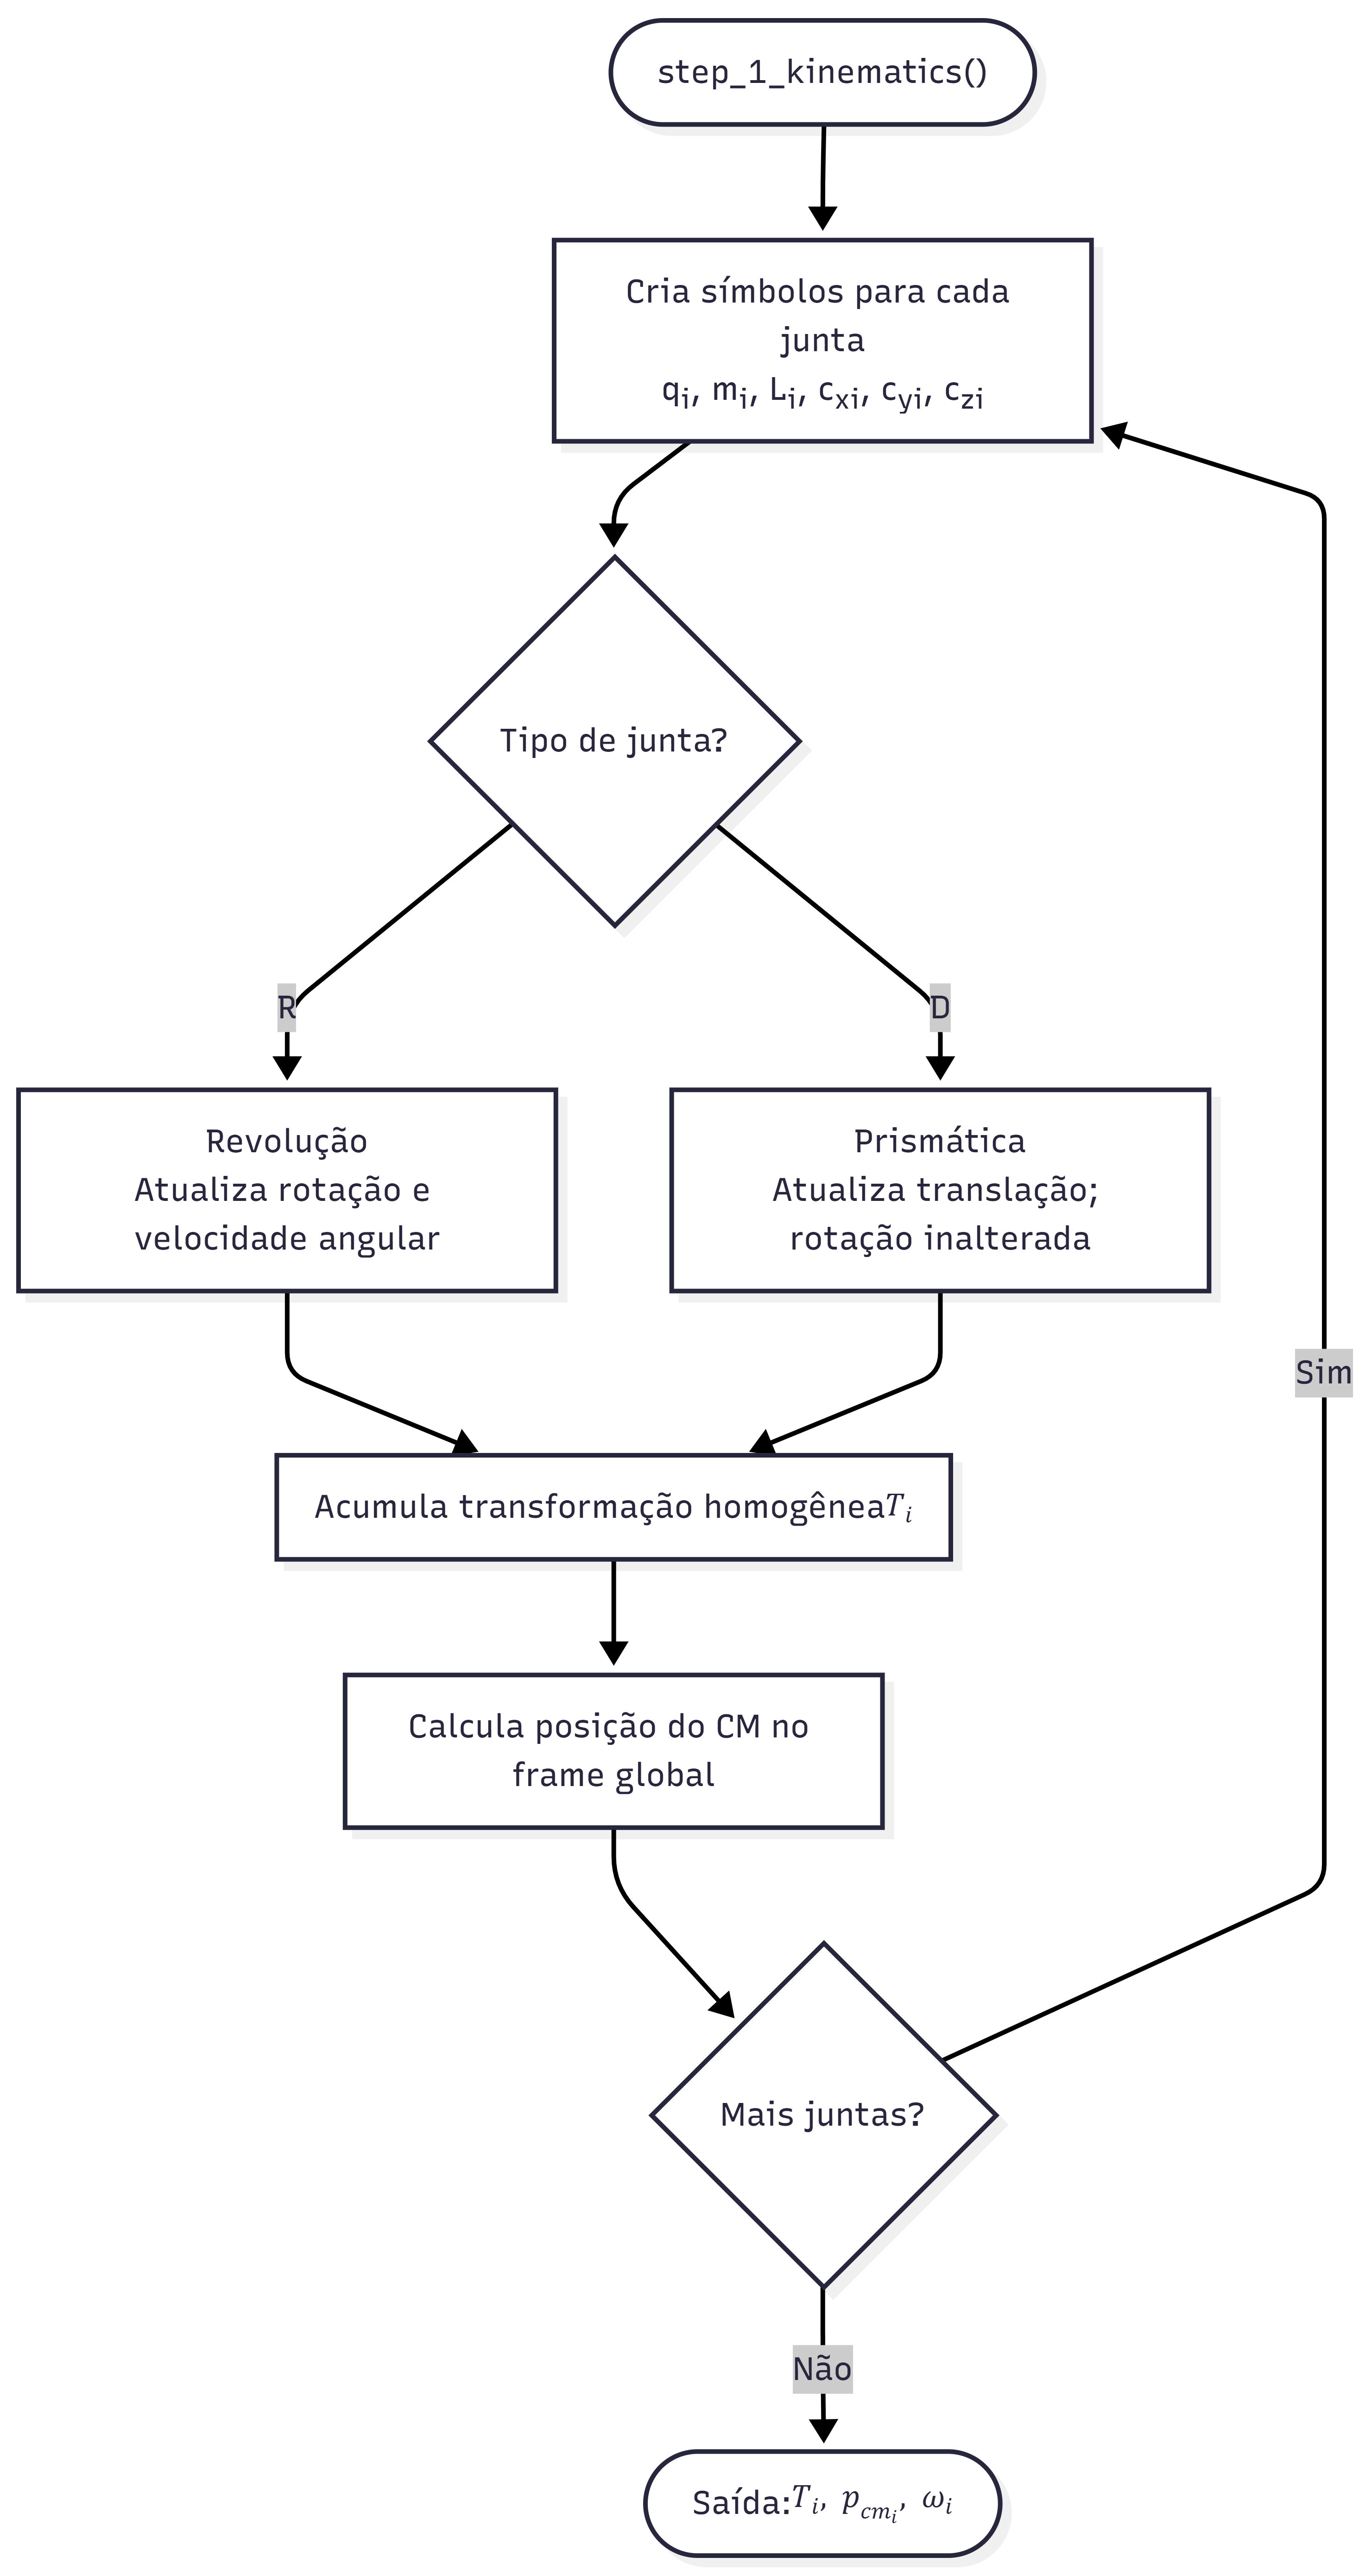
\includegraphics[width=0.70\textwidth]{figuras/Diagramas/Diagrama 2a — Cinemática Simbólica.png}
    \caption{Fluxo de cinemática simbólica implementado em \texttt{step\_1\_kinematics}: da especificação de \texttt{joint\_config} e \texttt{link\_vectors\_mask} à construção das transformações homogêneas acumuladas $T_i$, das posições dos centros de massa $\vec{p}_{\text{cm},i}$, das velocidades angulares $\vec{\omega}_i$ e do Jacobiano geométrico completo $J(q) \in \mathbb{R}^{6 \times N}$.}
    \label{fig:cinem_simbolica}
\end{figure}

% ==============================================================================
\section{Derivação Simbólica da Matriz de Inércia e do Vetor de Gravidade}
\label{sec:M_G}
% ==============================================================================

\subsection{Método do Jacobiano da Inércia}

A derivação da matriz de inércia generalizada $M(q)$ segue o método do Jacobiano da inércia \cite{siciliano2009robotics}, que expressa a energia cinética total como:
\begin{equation}
    T = \frac{1}{2}\dot{q}^\top M(q)\,\dot{q},
    \label{eq:T_total}
\end{equation}
onde:
\begin{itemize}
    \item $T \in \mathbb{R}$ é a energia cinética total do sistema;
    \item $\dot{q} \in \mathbb{R}^{N}$ é o vetor de velocidades generalizadas (uma componente por junta);
    \item $M(q) \in \mathbb{R}^{N\times N}$ é a matriz de inércia generalizada, simétrica e definida positiva;
    \item $N$ é o número de graus de liberdade da cadeia cinemática.
\end{itemize}

A matriz de inércia é construída pela soma das contribuições de cada elo:
\begin{equation}
    M(q) = \sum_{i=1}^{N} \left[ m_i\, J_{v,i}^\top\, J_{v,i} + J_{\omega,i}^\top\, I_i^{(g)}\, J_{\omega,i} \right].
    \label{eq:M_jacobian}
\end{equation}
onde:
\begin{itemize}
    \item $m_i \in \mathbb{R}$ é a massa do elo $i$;
    \item $J_{v,i} \in \mathbb{R}^{3\times N}$ é o Jacobiano de velocidade linear do centro de massa do elo $i$;
    \item $J_{\omega,i} \in \mathbb{R}^{3\times N}$ é o Jacobiano de velocidade angular do elo $i$;
    \item $I_i^{(g)} \in \mathbb{R}^{3\times 3}$ é o tensor de inércia do elo $i$ expresso no referencial global;
    \item $N$ é o número total de elos da cadeia.
\end{itemize}

Os Jacobianos de velocidade translacional e angular do CM do elo $i$ são obtidos diretamente por diferenciação simbólica:
\begin{equation}
    J_{v,i}(q) = \frac{\partial \vec{p}_{\text{cm},i}}{\partial q}, \qquad
    J_{\omega,i}(\dot{q}) = \frac{\partial \vec{\omega}_i}{\partial \dot{q}},
    \label{eq:jacobs}
\end{equation}
onde:
\begin{itemize}
    \item $J_{v,i}(q) \in \mathbb{R}^{3\times N}$ é o Jacobiano de velocidade linear do centro de massa do elo $i$;
    \item $J_{\omega,i}(\dot{q}) \in \mathbb{R}^{3\times N}$ é o Jacobiano de velocidade angular do elo $i$;
    \item $\vec{p}_{\text{cm},i} \in \mathbb{R}^{3}$ é a posição do CM do elo $i$ (Equação~\eqref{eq:pcm_global});
    \item $\vec{\omega}_i \in \mathbb{R}^{3}$ é a velocidade angular global do elo $i$ (Equação~\eqref{eq:omega_rec});
    \item $\partial/\partial q$ e $\partial/\partial \dot{q}$ denotam as derivadas parciais matriciais em relação aos vetores $q$ e $\dot{q}$.
\end{itemize}

Estas derivadas são computadas pelo método \texttt{.jacobian()} do SymPy. O tensor de inércia global $I_i^{(g)}$ é obtido pela transformação de Steiner:
\begin{equation}
    I_i^{(g)} = R_{\text{acc},i}\, I_i^{(l)}\, R_{\text{acc},i}^\top, \qquad
    I_i^{(l)} = \text{diag}(Ixx_i,\, Iyy_i,\, Izz_i),
    \label{eq:I_global}
\end{equation}
onde:
\begin{itemize}
    \item $I_i^{(g)} \in \mathbb{R}^{3\times 3}$ é o tensor de inércia do elo $i$ expresso no referencial global;
    \item $I_i^{(l)} \in \mathbb{R}^{3\times 3}$ é o tensor de inércia local, diagonal nas coordenadas principais do elo;
    \item $R_{\text{acc},i} \in \mathbb{R}^{3\times 3}$ é a matriz de rotação global acumulada até o elo $i$;
    \item $Ixx_i, Iyy_i, Izz_i$ são os momentos principais de inércia do elo no referencial local.
\end{itemize}
A hipótese de tensor diagonal em coordenadas principais locais , amplamente adotada quando os eixos de inércia são alinhados ao referencial de junta \cite{spong2020robot, siciliano2009robotics} , é suficiente para descrever elos com geometria simétrica.

\subsection{Vetor de Gradiente de Potencial Gravitacional}

A energia potencial total do sistema é:
\begin{equation}
    V(q) = \sum_{i=1}^{N} m_i\, g\, z_{\text{cm},i}(q),
    \label{eq:V_grav}
\end{equation}
onde:
\begin{itemize}
    \item $V(q) \in \mathbb{R}$ é a energia potencial gravitacional total do sistema;
    \item $m_i$ é a massa do elo $i$;
    \item $g$ é a aceleração da gravidade;
    \item $z_{\text{cm},i}(q)$ é a componente vertical (terceira coordenada) de $\vec{p}_{\text{cm},i}$, dependente da configuração $q$;
    \item $N$ é o número de elos.
\end{itemize}

O vetor de gravidade generalizada é então:
\begin{equation}
    G(q) = \left(\frac{\partial V}{\partial q}\right)^\top = \frac{\partial}{\partial q} \left[\sum_{i=1}^{N} m_i\, g\, z_{\text{cm},i}\right]^\top,
    \label{eq:G_vec}
\end{equation}
onde:
\begin{itemize}
    \item $G(q) \in \mathbb{R}^{N}$ é o vetor de torques generalizados devidos à gravidade;
    \item $\partial V/\partial q \in \mathbb{R}^{1\times N}$ é o gradiente da energia potencial em relação ao vetor de coordenadas generalizadas $q$;
    \item cada componente $G_i(q)$ representa o torque generalizado necessário para sustentar o peso estático do sistema na configuração $q$ \cite{craig1989introduction, spong2020robot};
    \item $(\cdot)^\top$ denota transposição, convertendo o gradiente-linha em vetor-coluna.
\end{itemize}
Esse vetor é computado pelo método \texttt{sp.Matrix([V\_tot]).jacobian(self.q).T}.

\subsection{Jacobiano Geométrico Completo}

O Jacobiano geométrico do efetuador $J(q) \in \mathbb{R}^{6 \times N}$ é montado pela concatenação das linhas translacionais (derivada da posição do extremo final em relação a $q$) com as linhas rotacionais (derivada de $\vec{\omega}_N$ em relação a $\dot{q}$):
\begin{equation}
    J(q) = \begin{bmatrix} J_{\text{lin}} \\ J_{\text{ang}} \end{bmatrix}, \quad
    J_{\text{lin}} = \frac{\partial\, \vec{p}_{\text{end}}}{\partial q} \in \mathbb{R}^{3 \times N}, \quad
    J_{\text{ang}} = \frac{\partial\, \vec{\omega}_N}{\partial \dot{q}} \in \mathbb{R}^{3 \times N}.
    \label{eq:jacobian_full}
\end{equation}
onde:
\begin{itemize}
    \item $J(q) \in \mathbb{R}^{6\times N}$ é o Jacobiano geométrico completo do efetuador;
    \item $J_{\text{lin}}$ é a parte linear, obtida pela derivada parcial da posição $\vec{p}_{\text{end}}$ do extremo final em relação a $q$;
    \item $J_{\text{ang}}$ é a parte angular, obtida pela derivada parcial da velocidade angular $\vec{\omega}_N$ do último elo em relação a $\dot{q}$;
    \item $\vec{p}_{\text{end}} \in \mathbb{R}^{3}$ é a posição cartesiana do efetuador no referencial global;
    \item $\vec{\omega}_N \in \mathbb{R}^{3}$ é a velocidade angular global do último elo da cadeia.
\end{itemize}

A disponibilidade do Jacobiano $6 \times N$ completo viabiliza o \emph{controle no espaço de tarefa 6D}, em que três coordenadas descrevem a \textbf{posição} cartesiana $(x, y, z)$ do efetuador e três coordenadas descrevem a sua \textbf{orientação} angular (\textit{roll}, \textit{pitch}, \textit{yaw}, ou, equivalentemente, o eixo-ângulo de uma rotação em $SO(3)$). As três primeiras linhas $J_{\text{lin}}$ projetam as velocidades de junta na velocidade linear do efetuador, enquanto as três últimas $J_{\text{ang}}$ as projetam na velocidade angular, totalizando seis graus de liberdade da tarefa cartesiana. Esta é uma extensão crítica em relação a abordagens que consideram apenas o Jacobiano posicional $3 \times N$, que são insuficientes para controle de orientação em tarefas de manipulação subaquática, soldagem, alinhamento com superfícies inclinadas ou inserção de peças, nas quais o ``onde'' (posição) e o ``como'' (orientação) do efetuador devem ser controlados simultaneamente \cite{chiaverini1997singularity, siciliano2009robotics}. O algoritmo de cinemática inversa em malha fechada que opera sobre este Jacobiano completo é detalhado na Seção~\ref{sec:clik_6d} do Capítulo~\ref{cap:simulacao}. O fluxo das Seções~\ref{sec:M_G} e~\ref{sec:cinematica_simbolica} é sintetizado na Figura~\ref{fig:dinam_simbolica}, na qual se evidencia como $M(q)$, $G(q)$ e $J(q)$ são derivados a partir das posições e Jacobianos de cada elo.

\begin{figure}[htbp]
    \centering
    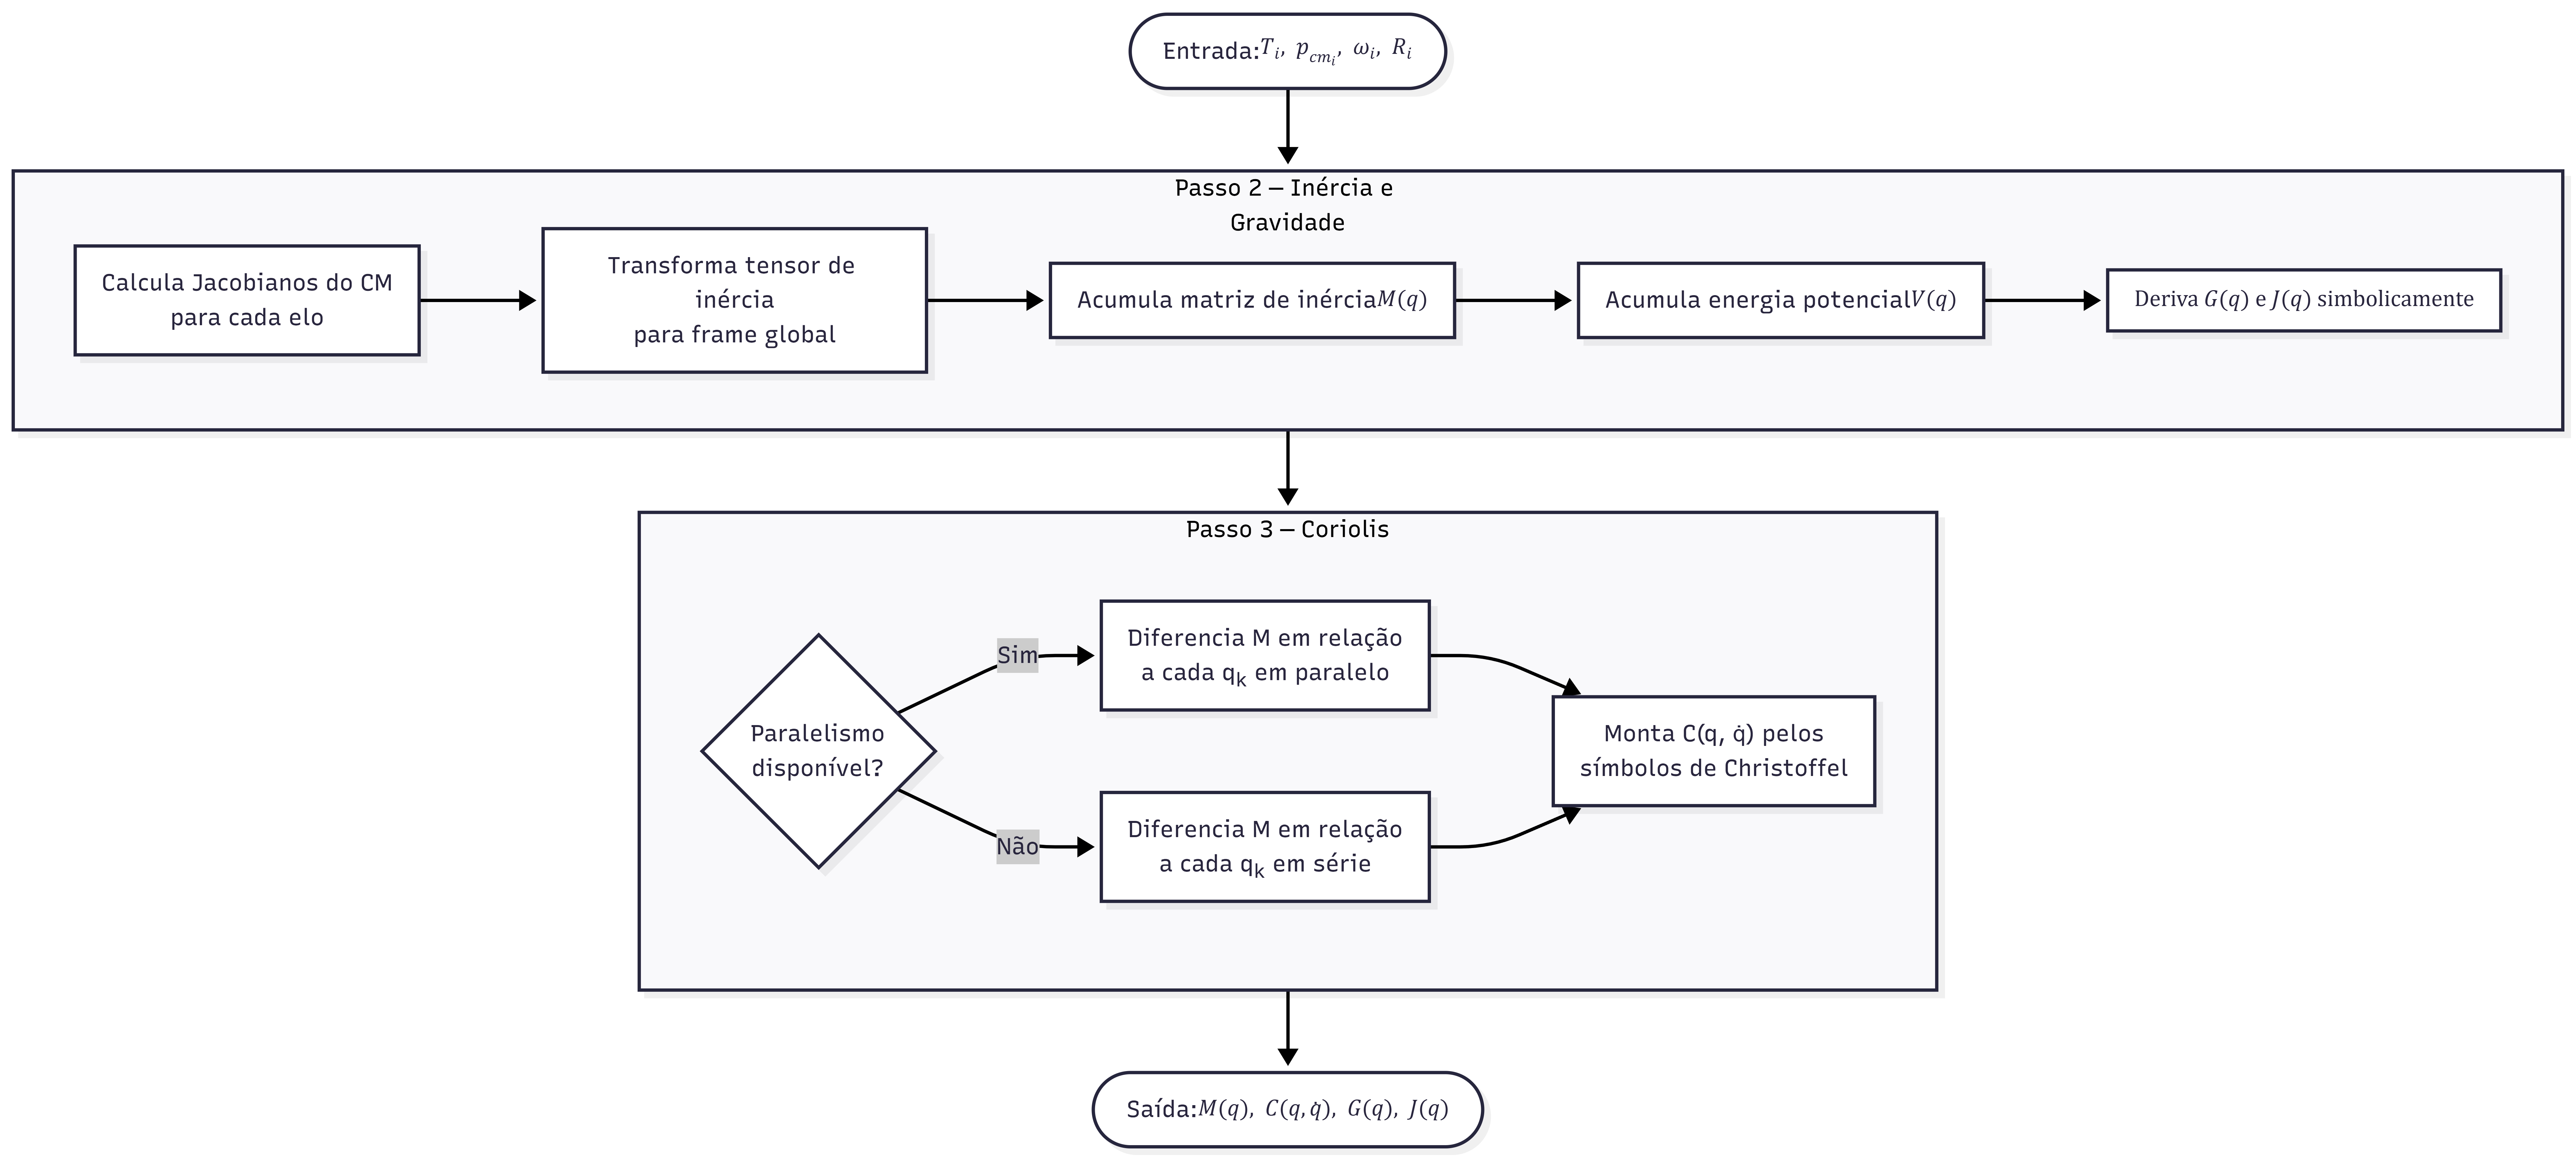
\includegraphics[width=0.92\textwidth]{figuras/Diagramas/Diagrama 2b — Dinâmica Simbólica M G e Coriolis.png}
    \caption{Fluxo de derivação simbólica da matriz de inércia $M(q)$, do vetor de gradiente de potencial $G(q)$ e dos coeficientes de Coriolis pelo método dos símbolos de Christoffel, implementado em \texttt{step\_2\_jacobian\_M\_G} e \texttt{step\_3\_coriolis\_combined}.}
    \label{fig:dinam_simbolica}
\end{figure}

% ==============================================================================
\section{Cálculo Simbólico do Vetor de Coriolis}
\label{sec:coriolis}
% ==============================================================================

\subsection{Formulação pelos Símbolos de Christoffel}

O vetor de termos de Coriolis e centrípetos $C(q,\dot{q}) \in \mathbb{R}^N$ é calculado pelos símbolos de Christoffel de segunda espécie \cite{spong2020robot, siciliano2009robotics}. Cada componente do vetor $C$ é:
\begin{equation}
    [C(q,\dot{q})]_i = \sum_{j=1}^{N}\sum_{k=j}^{N} c_{ijk}(q)\,\dot{q}_j\,\dot{q}_k \cdot \varepsilon_{jk},
    \label{eq:C_vec}
\end{equation}
onde:
\begin{itemize}
    \item $[C(q,\dot{q})]_i$ é a $i$-ésima componente do vetor de Coriolis;
    \item $c_{ijk}(q)$ são os símbolos de Christoffel de segunda espécie associados à matriz de inércia $M(q)$;
    \item $\dot{q}_j$ e $\dot{q}_k$ são velocidades generalizadas das juntas $j$ e $k$;
    \item $\varepsilon_{jk}$ é o coeficiente de simetria, com $\varepsilon_{jk} = 1$ se $j = k$ (termos centrípetos puros) e $\varepsilon_{jk} = 2$ se $j \neq k$ (termos de Coriolis cruzados);
    \item $N$ é o número de graus de liberdade.
\end{itemize}

Os coeficientes de Christoffel são:
\begin{equation}
    c_{ijk} = \frac{1}{2}\!\left(\frac{\partial M_{ij}}{\partial q_k} + \frac{\partial M_{ik}}{\partial q_j} - \frac{\partial M_{jk}}{\partial q_i}\right).
    \label{eq:christoffel_impl}
\end{equation}
onde:
\begin{itemize}
    \item $c_{ijk}(q) \in \mathbb{R}$ é o coeficiente de Christoffel de segunda espécie associado aos índices $(i,j,k)$;
    \item $M_{ij}, M_{ik}, M_{jk}$ são elementos da matriz de inércia $M(q)$;
    \item $\partial M_{ab}/\partial q_c$ é a derivada parcial do elemento $M_{ab}$ em relação à coordenada generalizada $q_c$.
\end{itemize}

Esta formulação é matematicamente equivalente às linhas $C_{ij}$ da matriz de Coriolis clássica (Equação~\eqref{eq:christoffel} do Capítulo~\ref{cap:revisao}), mas diretamente no formato vetorial $C(q,\dot{q})\dot{q}$, evitando a construção da matriz $N \times N$ completa , o que reduz o número total de operações de $O(N^3)$ para o cálculo dos coeficientes individuais sem custos adicionais de produto matriz-vetor.

A implementação segue dois sub-passos. No primeiro (\textit{Passo 3a}), a matriz de inércia $M$ é diferenciada em relação a cada variável de junta $q_k$, produzindo as matrizes $\partial M/\partial q_k \in \mathbb{R}^{N \times N}$ para $k = 1, \ldots, N$. No segundo (\textit{Passo 3b}), cada linha $i$ do vetor $C$ é montada pela varredura de todos os pares $(j, k)$ com $k \geq j$, utilizando as matrizes previamente calculadas. A exploração da simetria ($k \geq j$) reduz o número de pares de $N^2$ para $N(N+1)/2$ \cite{hollerbach1980recursive}.

\subsection{Estratégia de Paralelização da Derivação}

A derivação simbólica de $\partial M/\partial q_k$ é a operação mais custosa de toda a geração do modelo: em sistemas com $N$ graus de liberdade, cada um dos $N$ gradientes simbólicos exige a diferenciação de uma matriz $N \times N$ com entradas que podem possuir centenas de subexpressões, resultando em uma complexidade efetiva de $O(N^3)$ a $O(N^4)$ no tamanho das expressões para configurações gerais \cite{hollerbach1980recursive, leu1986automated}.

Para mitigar esse custo, o \textit{Hephaestus} distribui as $N$ tarefas de diferenciação $M \to \partial M/\partial q_k$ entre múltiplos processos via \texttt{ProcessPoolExecutor} da biblioteca padrão do Python:

\begin{equation}
    \texttt{dM\_dq}[k] = \frac{\partial M}{\partial q_k}, \quad k = 1, \ldots, N, \quad \text{computados em paralelo por } W \text{ \textit{workers}}.
    \label{eq:dMdq_parallel}
\end{equation}
onde:
\begin{itemize}
    \item $\texttt{dM\_dq}[k] \in \mathbb{R}^{N\times N}$ é a matriz de derivadas parciais $\partial M/\partial q_k$ armazenada na posição $k$ da lista resultante;
    \item $M \in \mathbb{R}^{N\times N}$ é a matriz de inércia simbólica completa;
    \item $q_k$ é a $k$-ésima coordenada generalizada;
    \item $N$ é o número de graus de liberdade;
    \item $W$ é o número de processos \textit{workers} alocados ao \texttt{ProcessPoolExecutor}.
\end{itemize}

O uso de processos (em vez de \textit{threads}) contorna a limitação do \textit{Global Interpreter Lock} (GIL) do CPython, que impede a execução simultânea de código Python puro em múltiplos \textit{threads} \cite{beazley2010understanding}. A serialização dos objetos simbólicos entre processos é viabilizada pela integração nativa do SymPy com o módulo \texttt{pickle} do Python, que representa expressões simbólicas como árvores de objetos serializáveis \cite{meurer2017sympy}.

Analogamente, o cálculo das $N$ linhas do vetor $C$ (cada linha requerendo $O(N^2)$ operações simbólicas sobre as matrizes $\partial M/\partial q_k$) é também paralelizado por \texttt{ProcessPoolExecutor}, com cada \textit{worker} responsável por uma linha $i$ do vetor:

\begin{equation}
    C_i = \sum_{j=1}^{N}\sum_{k=j}^{N} c_{ijk}\,\dot{q}_j\,\dot{q}_k \cdot \varepsilon_{jk}, \quad i = 1, \ldots, N, \quad \text{computados em paralelo}.
    \label{eq:C_parallel}
\end{equation}
onde:
\begin{itemize}
    \item $C_i$ é a $i$-ésima componente do vetor de Coriolis (cf.\ Equação~\eqref{eq:C_vec});
    \item $c_{ijk}$ são os coeficientes de Christoffel definidos pela Equação~\eqref{eq:christoffel_impl};
    \item $\dot{q}_j, \dot{q}_k$ são as velocidades generalizadas das juntas $j$ e $k$;
    \item $\varepsilon_{jk}$ é o coeficiente de simetria ($1$ ou $2$);
    \item $N$ é o número de graus de liberdade, e cada índice $i$ é processado por um \textit{worker} distinto.
\end{itemize}

Uma decisão de implementação relevante é a \emph{omissão intencional} da chamada a \texttt{sp.collect()} após a montagem de cada linha $C_i$. Embora a coleta de termos semelhantes possa compactar a expressão simbólica, seu custo computacional é superlinear no número de termos e pode superar em ordem de grandeza o custo do cálculo próprio da linha. Em vez disso, a compactação é delegada ao passo de CSE (\textit{Common Subexpression Elimination}) realizado posteriormente no \texttt{lambdify}, que fatoriza subexpressões repetidas de forma sistemática e com custo linear no tamanho da expressão final \cite{alfred2007compilers, meurer2017sympy}.

\subsection{Modo Serial para Ambientes Executáveis}

Quando o \textit{Hephaestus} é distribuído como executável via PyInstaller (arquivo \texttt{.exe}), o suporte ao \textit{spawn} de subprocessos no Windows impõe restrições de inicialização que tornam o \texttt{ProcessPoolExecutor} incompatível com módulos congelados (\textit{frozen}). Nesse cenário, o número de \textit{workers} é automaticamente configurado para 1, e a computação é realizada em série na mesma \textit{thread} principal. Essa detecção é realizada pelo parâmetro \texttt{num\_workers} da classe \texttt{RobotMathEngine}: quando \texttt{num\_workers = 1}, a condição \texttt{use\_parallel = False} desativa o executor, garantindo execução correta em qualquer ambiente sem modificações no código \cite{leu1986automated}.

% ==============================================================================
\section{Extensão Hidrodinâmica: \texttt{RobotMathHydro}}
\label{sec:hydro_engine}
% ==============================================================================

A classe \texttt{RobotMathHydro} herda integralmente de \texttt{RobotMathEngine} e sobrescreve os métodos \texttt{step\_1\_kinematics\_hydro} e \texttt{step\_2\_jacobian\_M\_G} para incorporar os efeitos físicos do ambiente aquático, conforme a formulação de Fossen \cite{fossen2011handbook} e Antonelli \cite{antonelli2014modelling}.

\subsection{Parâmetros Adicionais: Volumes e Massa Adicionada}

No passo de cinemática hidrodinâmica, após a execução completa de \texttt{step\_1\_kinematics}, são acrescentados à lista de parâmetros os volumes deslocados $\text{vol}_i$ de cada elo ($i = 1, \ldots, N$). Esses volumes determinam a força de empuxo por elo segundo o princípio de Arquimedes:
\begin{equation}
    B_i = \rho\, g\, \text{vol}_i,
    \label{eq:empuxo_por_elo}
\end{equation}
onde:
\begin{itemize}
    \item $B_i$ é o módulo da força de empuxo aplicada ao elo $i$;
    \item $\rho$ é a densidade do fluido (no caso típico, água do mar) \cite{newman1977marine};
    \item $g$ é a aceleração da gravidade;
    \item $\text{vol}_i$ é o volume submerso deslocado pelo elo $i$.
\end{itemize}

No passo de dinâmica hidrodinâmica, os coeficientes de massa adicionada de cada elo são instanciados como seis símbolos escalares:
\begin{equation}
    \{ma_{u,i},\, ma_{v,i},\, ma_{w,i}\} \quad \text{(translacionais)}, \qquad
    \{ma_{p,i},\, ma_{q,i},\, ma_{r,i}\} \quad \text{(rotacionais)},
    \label{eq:MA_syms}
\end{equation}
onde:
\begin{itemize}
    \item $ma_{u,i}, ma_{v,i}, ma_{w,i}$ são os coeficientes de massa adicionada translacionais nas direções $u$ (\textit{surge}), $v$ (\textit{sway}) e $w$ (\textit{heave}) do elo $i$, no referencial local;
    \item $ma_{p,i}, ma_{q,i}, ma_{r,i}$ são os coeficientes de massa adicionada rotacionais em torno dos eixos $p$ (\textit{roll}), $q$ (\textit{pitch}) e $r$ (\textit{yaw}) do elo $i$, no referencial local;
    \item o índice $i$ percorre todos os elos da cadeia ($i = 1, \ldots, N$).
\end{itemize}

Esses símbolos formam as matrizes diagonais locais $M_{A,\text{lin},i}^{(l)} = \text{diag}(ma_{u,i}, ma_{v,i}, ma_{w,i})$ e $M_{A,\text{rot},i}^{(l)} = \text{diag}(ma_{p,i}, ma_{q,i}, ma_{r,i})$. A parametrização diagonal é adequada para corpos com pelo menos um plano de simetria geométrica, condição satisfeita pela grande maioria dos elos de UVMSs comerciais \cite{fossen2011handbook}.

\subsection{Matriz de Inércia com Massa Adicionada}

A matriz de inércia generalizada no modo subaquático é:
\begin{equation}
    M_{\text{Hydro}}(q) = \sum_{i=1}^{N} \left[
        J_{v,i}^\top \left(m_i I_3 + M_{A,\text{lin},i}^{(g)}\right) J_{v,i}
        + J_{\omega,i}^\top \left(I_i^{(g)} + M_{A,\text{rot},i}^{(g)}\right) J_{\omega,i}
    \right],
    \label{eq:M_hydro_impl}
\end{equation}
onde:
\begin{itemize}
    \item $M_{\text{Hydro}}(q) \in \mathbb{R}^{N\times N}$ é a matriz de inércia generalizada no modo subaquático;
    \item $m_i$ é a massa do elo $i$ e $I_3$ é a matriz identidade $3\times 3$;
    \item $M_{A,\text{lin},i}^{(g)} \in \mathbb{R}^{3\times 3}$ é a matriz diagonal de massa adicionada translacional do elo $i$ no referencial global;
    \item $M_{A,\text{rot},i}^{(g)} \in \mathbb{R}^{3\times 3}$ é a matriz diagonal de massa adicionada rotacional do elo $i$ no referencial global;
    \item $I_i^{(g)} \in \mathbb{R}^{3\times 3}$ é o tensor de inércia rígida do elo $i$ no referencial global (Equação~\eqref{eq:I_global});
    \item $J_{v,i}, J_{\omega,i} \in \mathbb{R}^{3\times N}$ são os Jacobianos linear e angular do elo $i$ (Equação~\eqref{eq:jacobs}).
\end{itemize}

As matrizes de massa adicionada globais são obtidas pela transformação pelo referencial acumulado:
\begin{equation}
    M_{A,\text{lin},i}^{(g)} = R_{\text{acc},i}\, M_{A,\text{lin},i}^{(l)}\, R_{\text{acc},i}^\top, \qquad
    M_{A,\text{rot},i}^{(g)} = R_{\text{acc},i}\, M_{A,\text{rot},i}^{(l)}\, R_{\text{acc},i}^\top.
    \label{eq:MA_global}
\end{equation}
onde:
\begin{itemize}
    \item $M_{A,\text{lin},i}^{(l)}, M_{A,\text{rot},i}^{(l)} \in \mathbb{R}^{3\times 3}$ são as matrizes diagonais de massa adicionada translacional e rotacional no referencial local do elo $i$ (Equação~\eqref{eq:MA_syms});
    \item $R_{\text{acc},i} \in \mathbb{R}^{3\times 3}$ é a matriz de rotação global acumulada até o elo $i$;
    \item a transformação $R\,(\cdot)\,R^\top$ realiza a mudança de base de tensores de segunda ordem do referencial local para o global.
\end{itemize}

A Equação~\eqref{eq:M_hydro_impl} expande a Equação~\eqref{eq:M_jacobian} pelo princípio de superposição da inércia virtual \cite{fossen2011handbook}: a massa adicionada $M_{A,i}$ representa a inércia do fluido acelerado pelo movimento do elo $i$, projetada no espaço de juntas via Jacobianos, exatamente como a inércia rígida do próprio elo. Essa equivalência formal permite a reutilização do mesmo \textit{framework} de derivação de $M$ para ambos os cenários (ar e água), com mínima duplicação de código.

\subsection{Vetor de Potencial Aparente: Peso menos Empuxo}

A energia potencial aparente de cada elo submerso combina o potencial gravitacional com o trabalho da força de empuxo:
\begin{equation}
    V_i^{\text{app}}(q) = (m_i - \rho\, \text{vol}_i)\, g\, z_{\text{cm},i}(q),
    \label{eq:V_aparente}
\end{equation}
onde:
\begin{itemize}
    \item $V_i^{\text{app}}(q)$ é a energia potencial aparente (peso menos empuxo) do elo $i$;
    \item $m_i$ é a massa do elo $i$ e $\rho\, \text{vol}_i$ é a massa de fluido deslocada pelo elo;
    \item $g$ é a aceleração da gravidade;
    \item $z_{\text{cm},i}(q)$ é a coordenada vertical do CM do elo $i$;
    \item conforme definido na Equação~\eqref{eq:buoyancy_potential} do Capítulo~\ref{cap:revisao}.
\end{itemize}

O vetor $G_{\text{Hydro}}(q)$ resultante é o gradiente desta soma:
\begin{equation}
    G_{\text{Hydro}}(q) = \left(\frac{\partial}{\partial q} \sum_{i=1}^{N} (m_i - \rho\, \text{vol}_i)\,g\,z_{\text{cm},i}\right)^\top.
    \label{eq:G_hydro}
\end{equation}
onde:
\begin{itemize}
    \item $G_{\text{Hydro}}(q) \in \mathbb{R}^{N}$ é o vetor de torques generalizados aparentes (gravidade menos empuxo);
    \item os demais símbolos seguem a Equação~\eqref{eq:V_aparente};
    \item $(\cdot)^\top$ converte o gradiente-linha em vetor-coluna.
\end{itemize}

Quando $m_i \approx \rho\, \text{vol}_i$ (elo neutralmente flutuante), $V_i^{\text{app}} \approx 0$ e o correspondente torque estático $G_i(q)$ anula-se, reproduzindo o cenário típico de UVMSs projetados para equilíbrio neutro que minimizam o esforço estático dos atuadores \cite{antonelli2014modelling, yuh2001underwater}.

\subsection{Modelo Dinâmico Unificado}

A estrutura formal das equações de movimento hidrodinâmicas é idêntica à terrestre:
\begin{equation}
    M_{\text{Hydro}}(q)\ddot{q} + C_{\text{Hydro}}(q,\dot{q})\dot{q} + G_{\text{Hydro}}(q) = \tau,
    \label{eq:EOM_hydro}
\end{equation}
onde:
\begin{itemize}
    \item $M_{\text{Hydro}}(q) \in \mathbb{R}^{N\times N}$ é a matriz de inércia generalizada aparente (Equação~\eqref{eq:M_hydro_impl});
    \item $C_{\text{Hydro}}(q,\dot{q}) \in \mathbb{R}^{N\times N}$ é a matriz de Coriolis e termos centrípetos calculada pelos mesmos símbolos de Christoffel sobre $M_{\text{Hydro}}$ (Equação~\eqref{eq:christoffel_impl}), sem nenhuma modificação algorítmica;
    \item $G_{\text{Hydro}}(q) \in \mathbb{R}^{N}$ é o vetor de torques generalizados aparentes (Equação~\eqref{eq:G_hydro});
    \item $q, \dot{q}, \ddot{q} \in \mathbb{R}^{N}$ são os vetores de posições, velocidades e acelerações generalizadas;
    \item $\tau \in \mathbb{R}^{N}$ é o vetor de torques generalizados aplicados pelos atuadores.
\end{itemize} Os termos de arrasto hidrodinâmico $\tau_{\text{drag}} = D_{\text{lin}}\dot{q} + D_{\text{quad}}|\dot{q}|\dot{q}$ (Equação~\eqref{eq:drag} do Capítulo~\ref{cap:revisao}) são aplicados separadamente no integrador numérico como forças passivas, não na geração simbólica do modelo, pela razão de que sua forma $|\dot{q}_i|\dot{q}_i$ não é simbólica no sentido lagrangiano clássico \cite{fossen2011handbook}. Ilustra-se, na Figura~\ref{fig:hydro_extensao}, como \texttt{RobotMathHydro} estende \texttt{RobotMathEngine} por herança, sobrescrevendo os métodos de dinâmica para incorporar massa adicionada e potencial aparente Peso--Empuxo.

\begin{figure}[htbp]
    \centering
    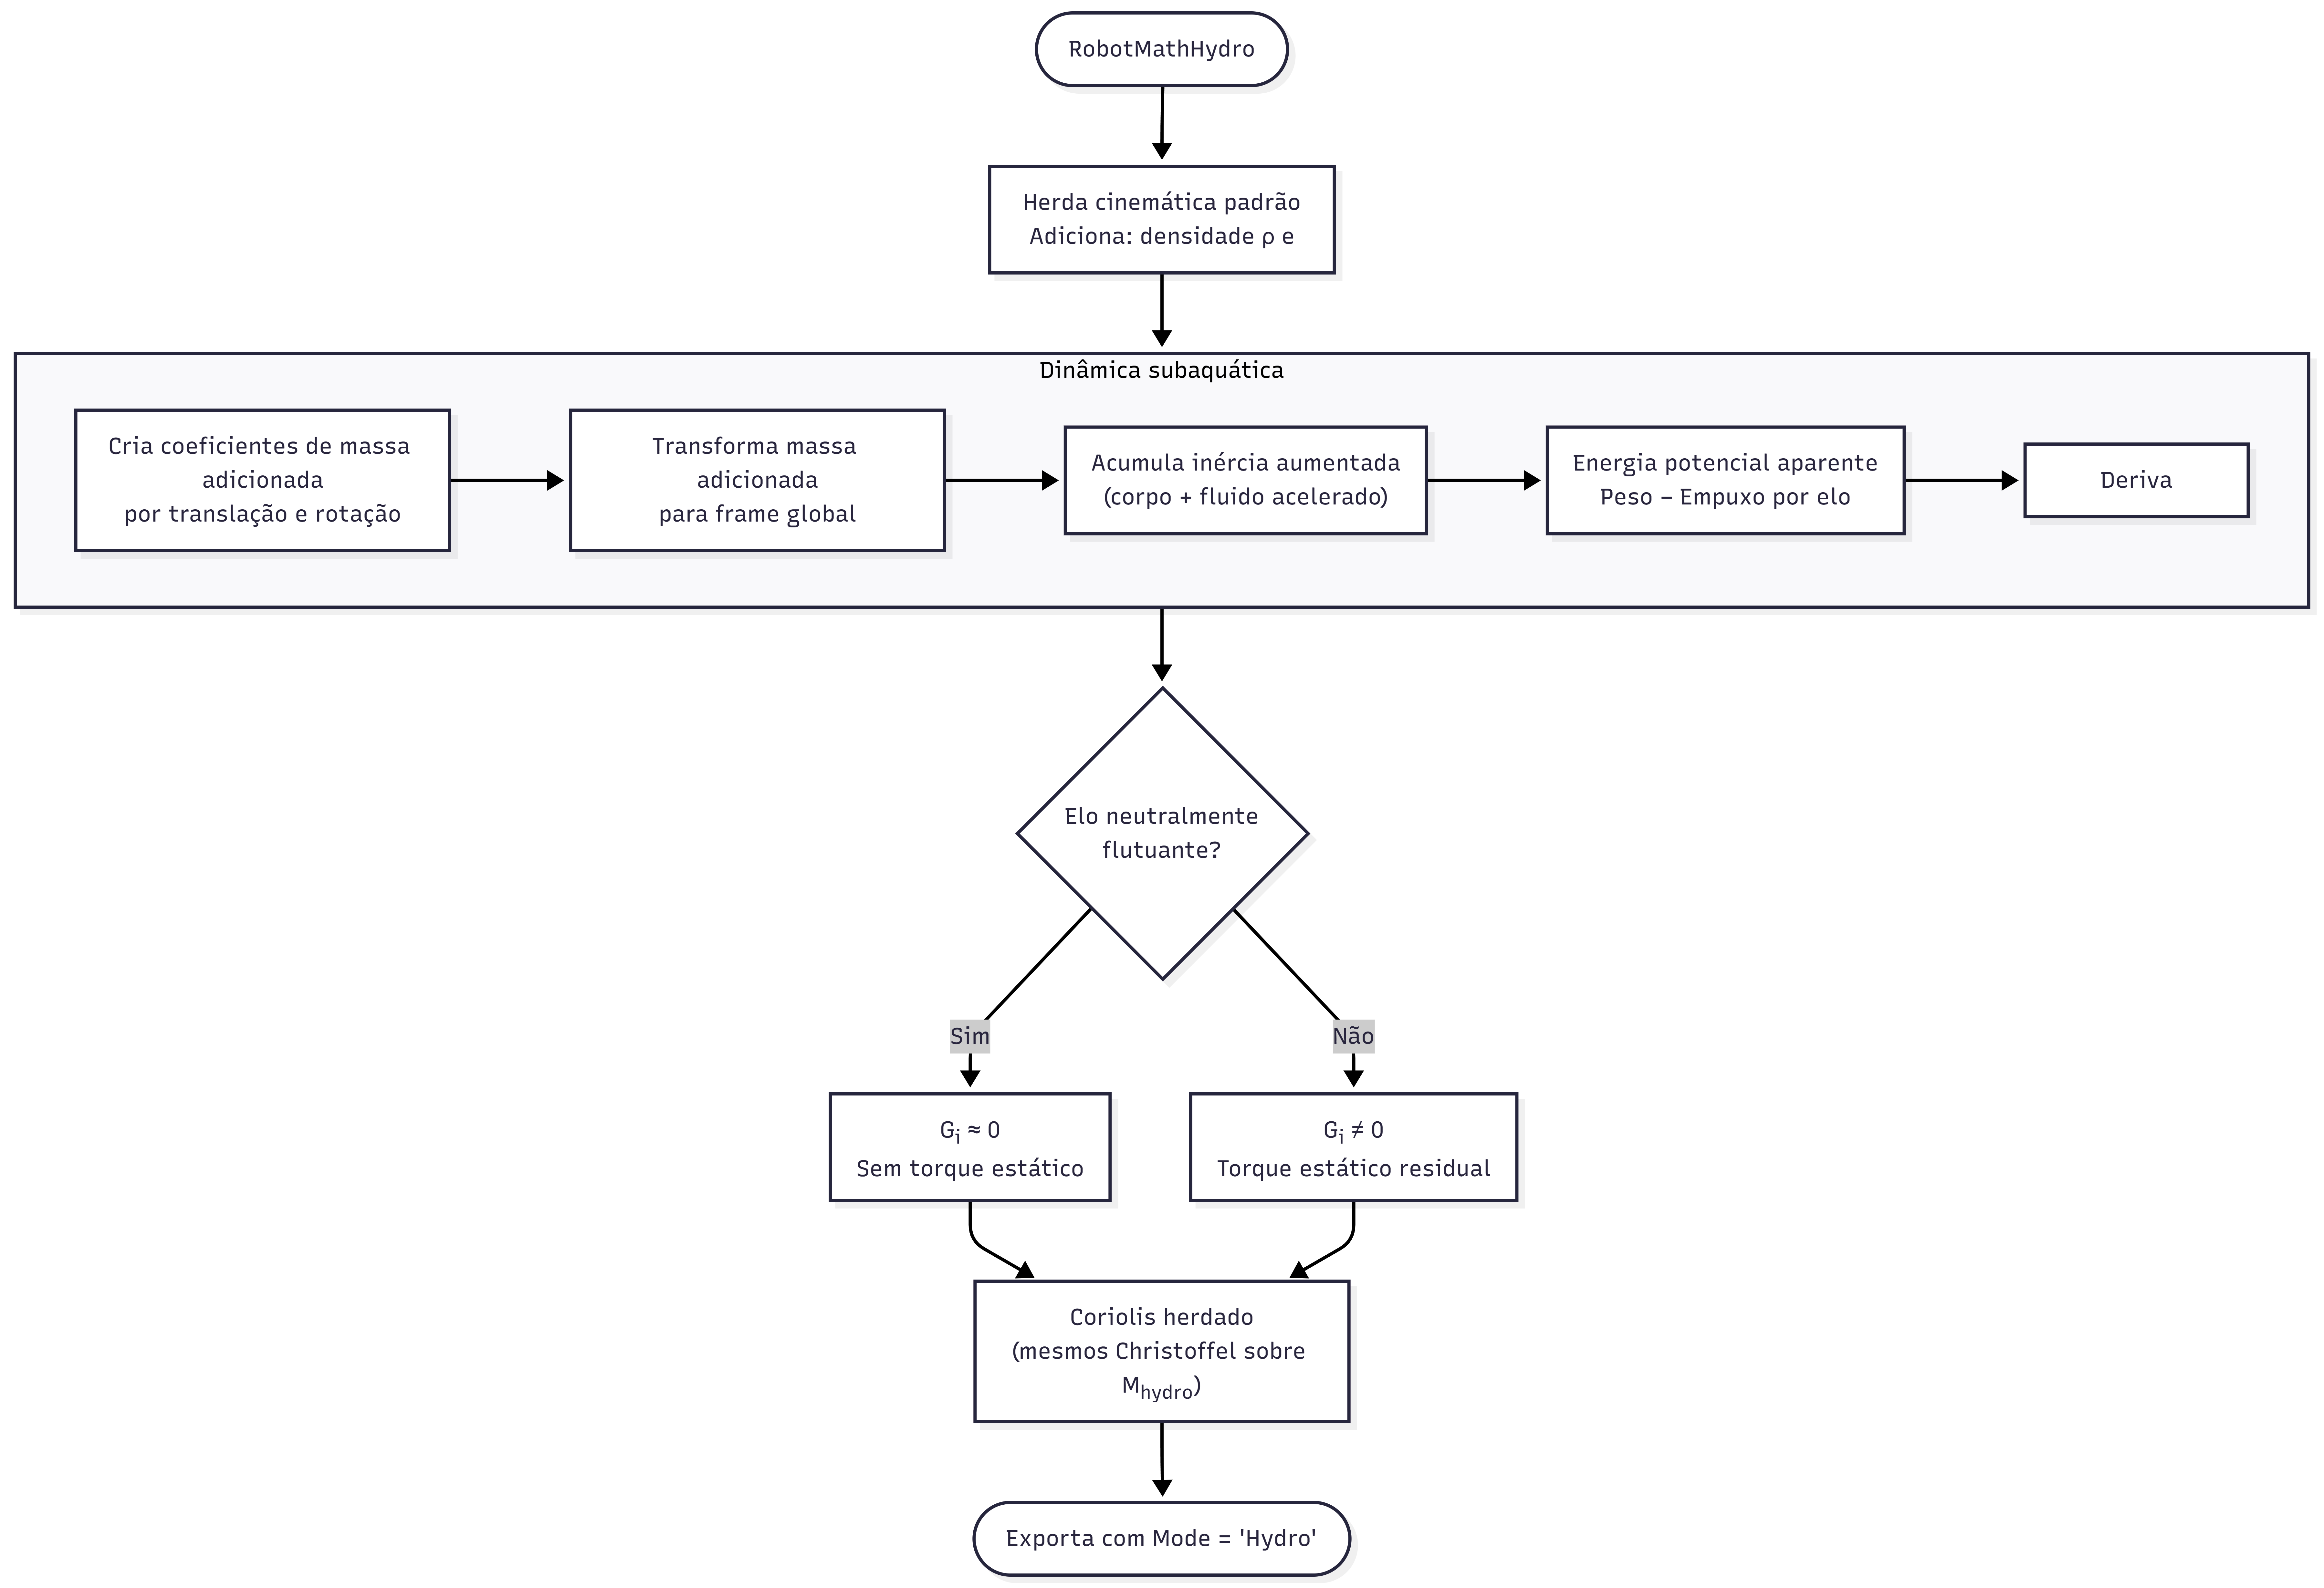
\includegraphics[width=1\textwidth]{figuras/Diagramas/Diagrama 3 — Extensão Hidrodinâmica.png}
    \caption{Extensão hidrodinâmica implementada em \texttt{RobotMathHydro}: herança de \texttt{RobotMathEngine} com sobrescrita dos métodos de cinemática e dinâmica para incorporar o tensor de massa adicionada $M_A^{(g)}$ (Equação~\eqref{eq:M_hydro_impl}) e o potencial aparente Peso--Empuxo (Equação~\eqref{eq:V_aparente}) segundo a formulação de Fossen~\cite{fossen2011handbook}.}
    \label{fig:hydro_extensao}
\end{figure}

% ==============================================================================
\section{Preparação e Exportação do Modelo Simbólico}
\label{sec:export}
% ==============================================================================

\subsection{Substituição de Símbolos Dinâmicos}

O método \texttt{step\_4\_prepare\_export} realiza a substituição dos \texttt{dynamicsymbols} dependentes do tempo , $q_i(t)$ e $\dot{q}_i(t)$ , por símbolos escalares estáticos $q_i$ e $\dot{q}_i$, via o mapeamento:
\begin{equation}
    q_i(t) \mapsto \texttt{sp.Symbol}(f\text{'q\{i\}'}), \qquad
    \dot{q}_i(t) \mapsto \texttt{sp.Symbol}(f\text{'dq\{i\}'}).
    \label{eq:subs_dynamic}
\end{equation}
onde:
\begin{itemize}
    \item $q_i(t)$ é a função simbólica dependente do tempo, criada via \texttt{dynamicsymbols} do SymPy;
    \item $\dot{q}_i(t) = dq_i(t)/dt$ é sua derivada temporal simbólica;
    \item $\mapsto$ representa a substituição da função do tempo por um símbolo escalar livre;
    \item $\texttt{sp.Symbol}(\cdot)$ é o construtor de símbolos escalares estáticos do SymPy;
    \item $f\text{'q\{i\}'}$ e $f\text{'dq\{i\}'}$ são os nomes \textit{formatados} das variáveis estáticas (e.g., \texttt{q1}, \texttt{dq1}, \texttt{q2}, \ldots).
\end{itemize}

Esse passo é necessário porque \texttt{dynamicsymbols} são, internamente, funções do tempo no SymPy, e sua presença nas expressões interfere com o \texttt{lambdify} , que espera símbolos escalares como variáveis de entrada \cite{meurer2017sympy}. A substituição não altera a estrutura algébrica das expressões; apenas troca a representação interna de ``função aplicada'' para ``símbolo livre''.

\subsection{Exportação do Dicionário de Resultados}

O método retorna um dicionário com as seguintes chaves:

\begin{itemize}
    \item \texttt{"M"}: a matriz de inércia $M(q) \in \mathbb{R}^{N \times N}$, expressa nos símbolos estáticos;
    \item \texttt{"G"}: o vetor de gradiente de potencial $G(q) \in \mathbb{R}^N$;
    \item \texttt{"C"}: o vetor de Coriolis $C(q,\dot{q}) \in \mathbb{R}^N$ (já no formato $C(q,\dot{q})\dot{q}$);
    \item \texttt{"J"}: o Jacobiano geométrico $J(q) \in \mathbb{R}^{6 \times N}$;
    \item \texttt{"FK\_Pos"}: a transformação homogênea completa do efetuador final $T_N(q)$;
    \item \texttt{"FK\_Vel"}: a velocidade cartesiana do efetuador $J(q)\dot{q}$;
    \item \texttt{"Subs"}: o mapeamento de substituição (Equação~\eqref{eq:subs_dynamic});
    \item \texttt{"Mode"}: string \texttt{"Air"} ou \texttt{"Hydro"}, para controle de fluxo no simulador.
\end{itemize}

Essa interface de exportação desacopla completamente a \textit{engine} matemática do módulo de simulação, permitindo que o modelo simbólico seja serializado (via \texttt{pickle}) e reutilizado em sessões posteriores sem recomputação , uma funcionalidade de produtividade crítica, dado que a geração do modelo para sistemas com $N \geq 6$ pode levar dezenas de minutos em \textit{hardware} convencional \cite{leu1986automated, hollerbach1980recursive}.

% ==============================================================================
\section{Compilação Simbólico-Numérica com \texttt{lambdify} e CSE}
\label{sec:lambdify_cse}
% ==============================================================================

\subsection{A Interface \texttt{lambdify}}

A transição das expressões simbólicas para funções numéricas avaliáveis é o passo de maior impacto sobre o desempenho computacional da simulação. O SymPy fornece a função \texttt{sp.lambdify()} para esse propósito: dado um conjunto de variáveis simbólicas $\{v_1, \ldots, v_k\}$ e uma expressão (ou matriz) simbólica $\mathcal{E}(v_1,\ldots,v_k)$, \texttt{lambdify} gera o código-fonte Python/NumPy equivalente e compila-o via \texttt{exec}, retornando uma função numérica de alta performance \cite{meurer2017sympy}.

No \textit{Hephaestus}, a assinatura do \texttt{lambdify} é:
\begin{equation}
    f_{M,C,G,J}(q_1,\ldots,q_N,\,\dot{q}_1,\ldots,\dot{q}_N,\,g,\,m_1,\,L_1,\,cx_1,\ldots) \to \mathbb{R}^{\cdot \times \cdot},
    \label{eq:lambdify_signature}
\end{equation}
onde:
\begin{itemize}
    \item $f_{M,C,G,J}$ representa cada uma das funções numéricas compiladas (uma para $M$, $C$, $G$ e $J$);
    \item $q_1, \ldots, q_N$ são as coordenadas generalizadas (entradas dinâmicas);
    \item $\dot{q}_1, \ldots, \dot{q}_N$ são as velocidades generalizadas;
    \item $g$ é a aceleração da gravidade;
    \item $m_1, L_1, cx_1, \ldots$ representam os parâmetros físicos (massa, comprimento, coordenadas do CM, momentos de inércia etc.) listados em \texttt{params\_list};
    \item $\mathbb{R}^{\cdot \times \cdot}$ denota a saída numérica, cuja dimensão depende da grandeza avaliada (e.g., $N\times N$ para $M$, $N$ para $G$, $6\times N$ para $J$).
\end{itemize}
Essa assinatura corresponde à lista \texttt{sym\_vars = bot.q + bot.dq + bot.params\_list}, e garante que a mesma assinatura seja utilizada para todas as funções compiladas ($M$, $C$, $G$, $J$, FK), simplificando o gerenciamento de argumentos no \textit{loop} de simulação.

\subsection{Eliminação de Subexpressões Comuns}

O parâmetro \texttt{cse=True} ativa a Eliminação de Subexpressões Comuns (\textit{Common Subexpression Elimination}, CSE) antes da geração do código numérico \cite{alfred2007compilers}. Internamente, o SymPy aplica o algoritmo de Risch-Moses para CSE \cite{moses1971algebraic}, identificando subárvores repetidas na expressão simbólica e substituindo cada ocorrência por uma variável temporária. O código Python gerado tem então a forma:

\begin{align}
    &\texttt{x0} = \sin(q_1), \quad \texttt{x1} = \cos(q_1), \quad \texttt{x2} = \texttt{x0} \cdot m_1, \quad \ldots \nonumber \\
    &M[0,0] = \texttt{x2} \cdot L_1^2 + \ldots, \quad M[0,1] = \texttt{x1} \cdot \texttt{x2} + \ldots
    \label{eq:cse_example}
\end{align}
onde:
\begin{itemize}
    \item $\texttt{x0}, \texttt{x1}, \texttt{x2}, \ldots$ são variáveis temporárias geradas pelo CSE para subexpressões repetidas;
    \item $\sin(q_1), \cos(q_1)$ são funções trigonométricas elementares avaliadas uma única vez por passo;
    \item $m_1, L_1$ são parâmetros físicos do primeiro elo (massa e comprimento);
    \item $M[0,0], M[0,1]$ são elementos da matriz de inércia compilada, expressos em função das variáveis temporárias e dos parâmetros físicos.
\end{itemize}

O impacto quantitativo da CSE é substancial: para um manipulador de 6 GDL em ar, a expressão simbólica de $M(q)$ pode conter $O(10^3)$ a $O(10^4)$ operações primitivas; com CSE, a função compilada executa tipicamente $2$--$5\times$ mais rápido, com redução de $60$--$90\%$ no tamanho do \textit{bytecode} \cite{meurer2017sympy, alfred2007compilers}. Para sistemas maiores ($N > 8$), a CSE pode ser a diferença entre uma compilação que produz código de tamanho manejável e uma que gera \textit{strings} de vários MB que excedem os limites de compilação do Python (\texttt{MemoryError}) \cite{leu1986automated}.

Adicionalmente, o módulo \texttt{modules='numpy'} instrui o \texttt{lambdify} a mapear funções simbólicas (\texttt{sp.sin}, \texttt{sp.cos}, etc.) para suas contrapartes NumPy (\texttt{np.sin}, \texttt{np.cos}), que por sua vez invocam implementações C compiladas via BLAS/LAPACK \cite{meurer2017sympy}. O resultado é uma função numérica que se comporta como código C nativo para as operações de ponto flutuante, sem o \textit{overhead} da álgebra simbólica em tempo de simulação.

\subsection{Compilação das Funções por Módulo}

No construtor \texttt{RobotSimulator.\_\_init\_\_}, cada grandeza dinâmica é compilada individualmente, produzindo quatro funções distintas:

\begin{itemize}
    \item \texttt{func\_M}: $f_M: \mathbb{R}^{2N+P} \to \mathbb{R}^{N \times N}$, avalia a matriz de inércia;
    \item \texttt{func\_C}: $f_C: \mathbb{R}^{2N+P} \to \mathbb{R}^{N}$, avalia o vetor de Coriolis;
    \item \texttt{func\_G}: $f_G: \mathbb{R}^{2N+P} \to \mathbb{R}^{N}$, avalia o gradiente de potencial;
    \item \texttt{func\_J}: $f_J: \mathbb{R}^{2N+P} \to \mathbb{R}^{6 \times N}$, avalia o Jacobiano completo;
    \item \texttt{funcs\_fk\_all\_links}: lista de $N$ funções $f_{\text{FK},i}: \mathbb{R}^{2N+P} \to \mathbb{R}^{3}$, avaliando a posição 3D do extremo do elo $i$ , utilizadas para a visualização gráfica animada do manipulador.
\end{itemize}

onde $P = |\texttt{params\_list}|$ é o número total de parâmetros físicos. A compilação separada por grandeza , em vez de uma única função monolítica , permite o despacho paralelo de $M$, $C$ e $G$ durante a simulação: cada uma das funções pode ser submetida simultaneamente a um \textit{worker} distinto do executor paralelo, triplicando a taxa de avaliação dinâmica em máquinas com pelo menos três núcleos \cite{leu1986automated}. Sintetiza-se, na Figura~\ref{fig:compilacao_simbolica}, o fluxo completo de compilação simbólico-numérica, desde as expressões SymPy geradas nas etapas anteriores até as funções NumPy prontas para avaliação a cada passo de integração.

\begin{figure}[htbp]
    \centering
    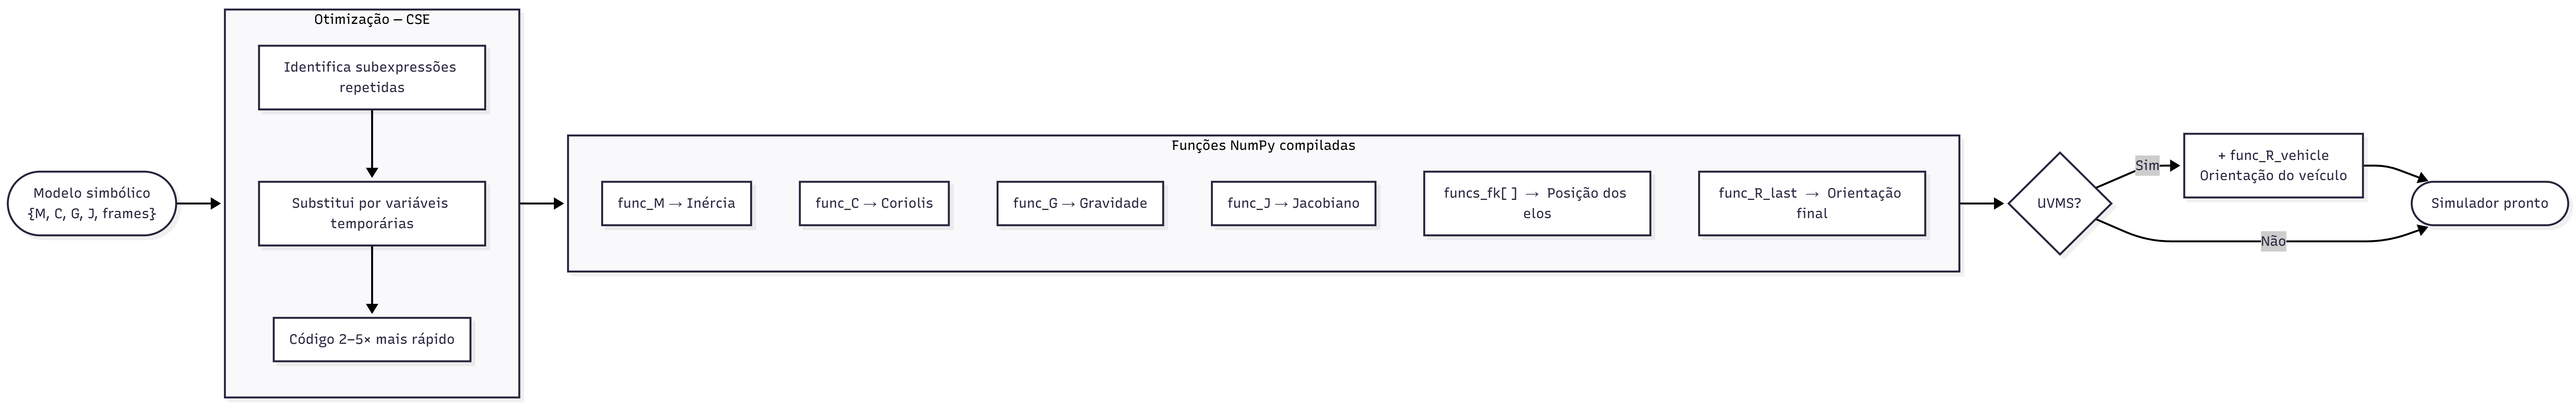
\includegraphics[width=0.92\textwidth]{figuras/Diagramas/Diagrama 4 — Compilação Simbólico-Numérica.png}
    \caption{Fluxo de compilação simbólico-numérica via \texttt{sp.lambdify()} com CSE ativo: as expressões SymPy de $M$, $C$, $G$ e $J$ passam pela Eliminação de Subexpressões Comuns antes de gerar código Python/NumPy compilado, reduzindo em 60--90\% o número de operações primitivas e viabilizando a avaliação em tempo de simulação \cite{meurer2017sympy, alfred2007compilers}.}
    \label{fig:compilacao_simbolica}
\end{figure}

% ==============================================================================
\section{Paralelismo em Dois Níveis e Executor Persistente}
\label{sec:parallel}
% ==============================================================================

O \textit{Hephaestus} implementa paralelismo em dois níveis distintos, correspondentes às duas fases temporalmente separadas do fluxo de trabalho:

\subsection{Nível 1: Paralelismo na Derivação Simbólica}

Como descrito na Seção~\ref{sec:coriolis}, o cálculo de $\partial M/\partial q_k$ e das linhas de $C$ é distribuído entre múltiplos processos durante a fase de \emph{geração do modelo} (executada uma única vez). O custo de \textit{spawn} dos processos e da serialização das expressões simbólicas é amortizado pelo ganho de velocidade na derivação, sendo lucrativo quando $N \geq 4$ e $W \geq 2$ processos estão disponíveis \cite{hollerbach1980recursive, beazley2010understanding}.

\subsection{Nível 2: Paralelismo na Avaliação Numérica}

Durante a fase de \emph{simulação}, as funções \texttt{func\_M}, \texttt{func\_C} e \texttt{func\_G} são avaliadas numericamente a cada passo de integração física (tipicamente $\Delta t = 10^{-3}$ s, correspondendo a 1000 avaliações por segundo de simulação). Para evitar o custo de \textit{respawn} de processos a cada avaliação , que, em testes, somava 2-8 segundos por simulação , o \textit{Hephaestus} utiliza um \textbf{executor persistente} (\texttt{ProcessPoolExecutor} pré-inicializado):

\begin{itemize}
    \item O executor é instanciado \emph{uma única vez} após a compilação, por meio do método \texttt{warm\_up\_workers()}, e mantido ativo durante toda a vida do objeto \texttt{RobotSimulator};
    \item Cada \textit{worker} executa o \textit{inicializador} \texttt{\_init\_worker}, que compila localmente as expressões simbólicas (via \texttt{lambdify}) e armazena as funções no dicionário de módulo \texttt{\_WORKER\_FUNCS};
    \item A cada passo de simulação, três tarefas são submetidas ao executor em paralelo , \texttt{("M", args)}, \texttt{("C", args)}, \texttt{("G", args)} , e os resultados são coletados por \texttt{Future.result()};
    \item O executor é encerrado explicitamente pelo método \texttt{close()}, chamado automaticamente no protocolo de fechamento da interface gráfica (\texttt{on\_closing}).
\end{itemize}

A abordagem de executor persistente com compilação nos \textit{workers} (em vez de serialização das funções compiladas, que o \texttt{pickle} não suporta) elimina o custo de \textit{respawn} e reduz o \textit{overhead} de IPC (\textit{Inter-Process Communication}) a apenas a serialização dos argumentos numéricos (vetores de ponto flutuante), que é negligenciável \cite{beazley2010understanding}.

Quando o paralelismo não está ativo (\texttt{use\_parallel=False}), as três funções são avaliadas sequencialmente na \textit{thread} principal, sem instanciar o executor , comportamento padrão seguro para qualquer ambiente de execução, incluindo executáveis PyInstaller. Ilustram-se, na Figura~\ref{fig:paralelismo_2niveis}, os dois níveis de paralelismo, suas fronteiras temporais distintas e os papéis do \texttt{ProcessPoolExecutor} em cada fase do ciclo de vida do \textit{Hephaestus}.

\begin{figure}[htbp]
    \centering
    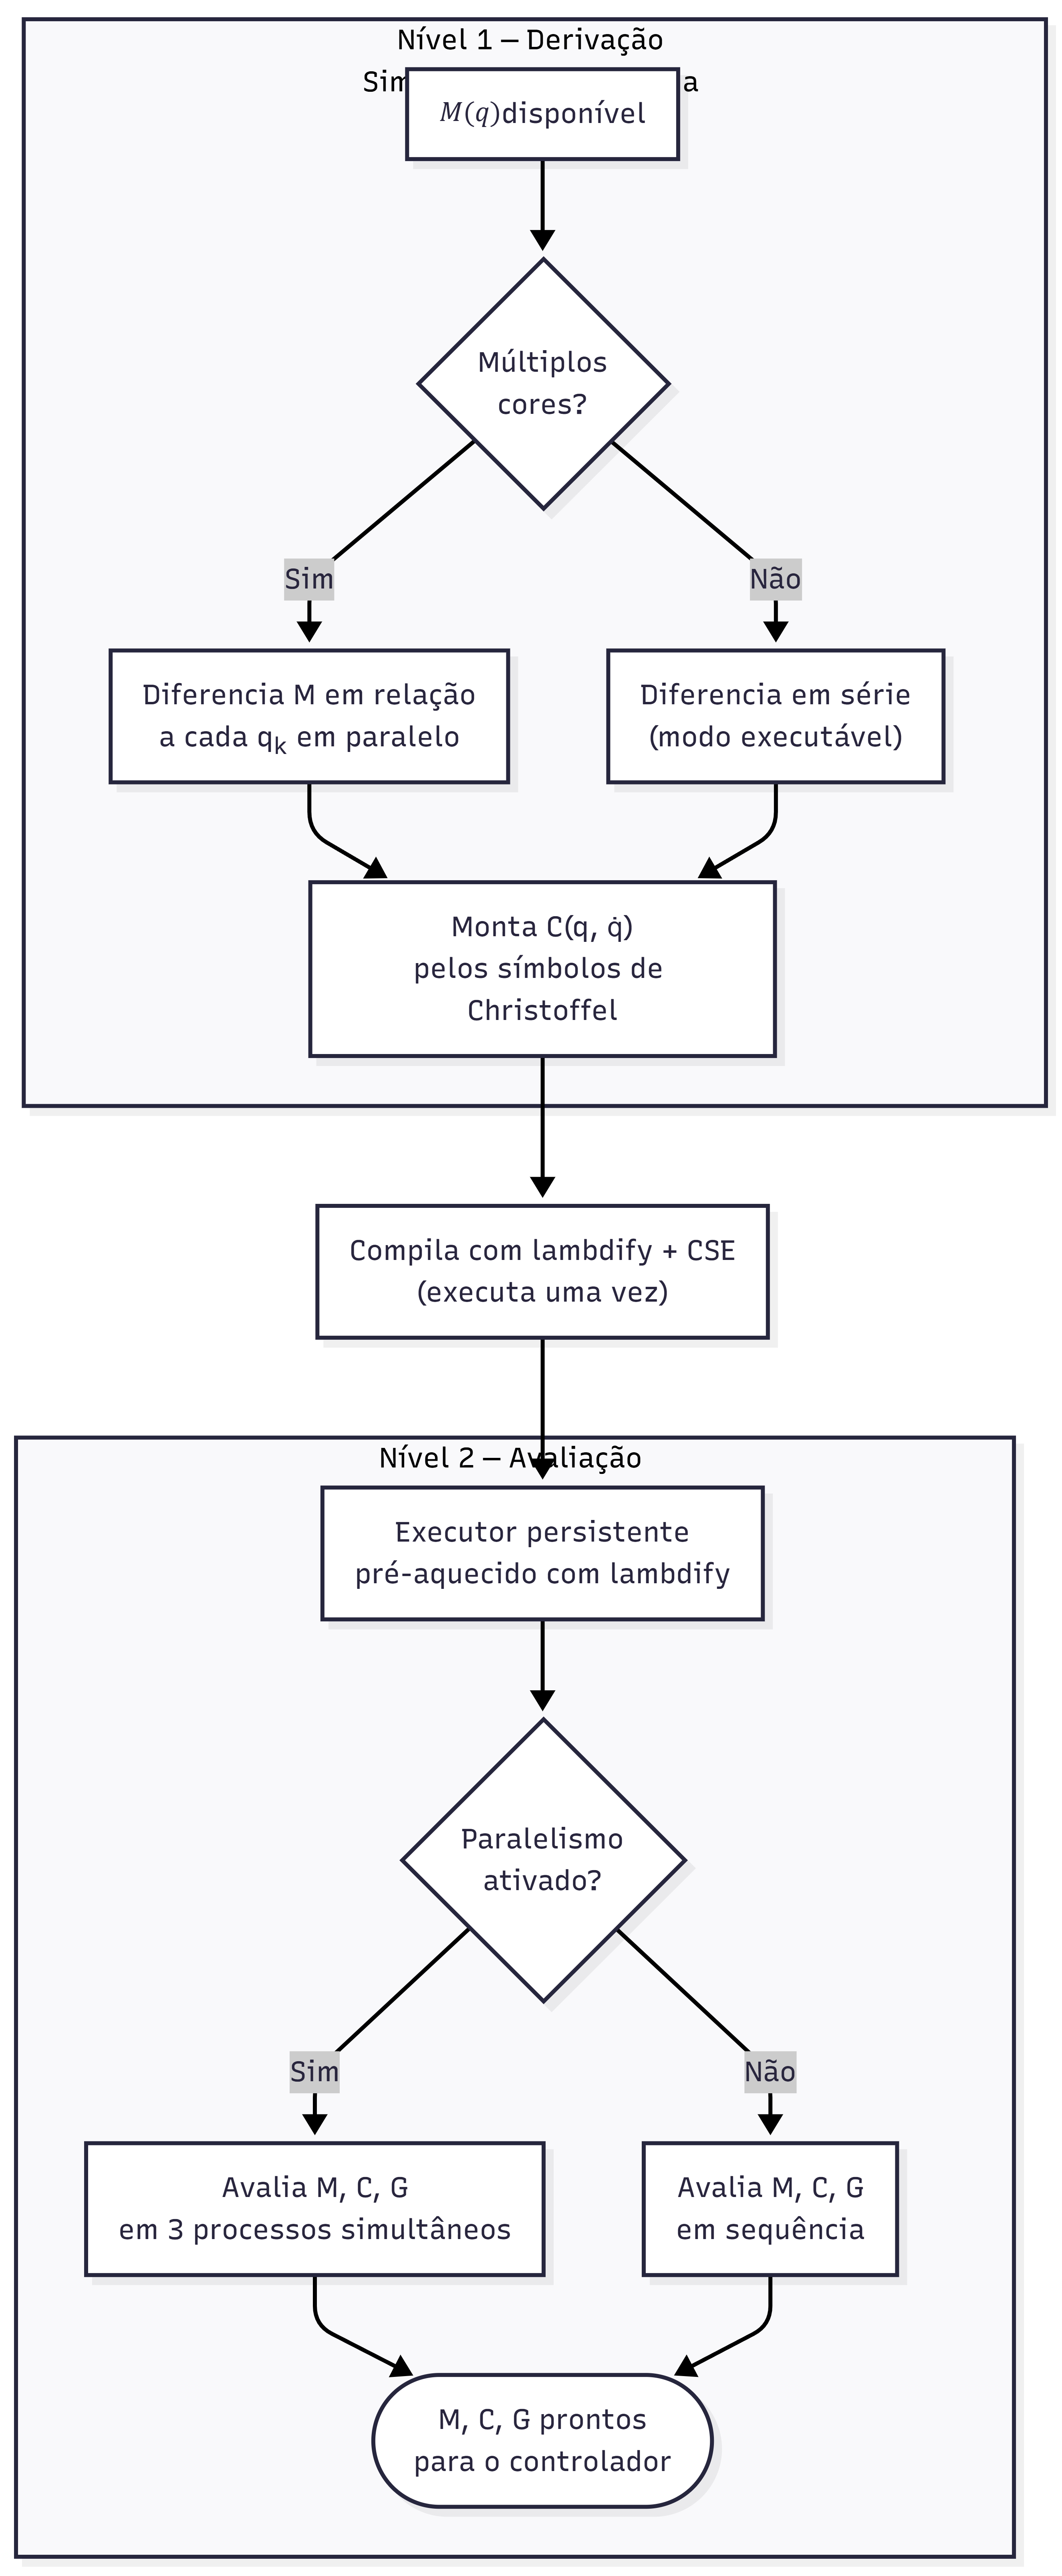
\includegraphics[width=0.5\textwidth]{figuras/Diagramas/Diagrama 12 — Paralelismo em Dois Níveis.png}
    \caption{Paralelismo em dois níveis no \textit{Hephaestus}: (Nível~1) derivação paralela de $\partial M/\partial q_k$ e das linhas de $C$ por \texttt{ProcessPoolExecutor} durante a geração \textit{offline} do modelo; (Nível~2) avaliação paralela e persistente de \texttt{func\_M}, \texttt{func\_C} e \texttt{func\_G} a cada passo de integração física durante a simulação \textit{online}.}
    \label{fig:paralelismo_2niveis}
\end{figure}

% ==============================================================================
\section{Considerações sobre a Complexidade Computacional}
\label{sec:complexidade}
% ==============================================================================

Resume-se, na Tabela~\ref{tab:complexidade}, a complexidade computacional das etapas de modelagem e simulação do \textit{Hephaestus}, comparada com as referências clássicas da literatura.

\begin{table}[h!]
\centering
\caption{Complexidade computacional das etapas de modelagem e simulação.}
\label{tab:complexidade}
\begin{tabular}{p{4.8cm} p{3.5cm} p{5.5cm}}
\hline
\textbf{Etapa} & \textbf{Complexidade} & \textbf{Referência / Observação} \\
\hline
Cinemática FK simbólica & $O(N^2)$ & Produto acumulado de matrizes $4\times4$ \cite{craig1989introduction} \\
Derivação de $M(q)$ (simbólica) & $O(N^3)$ & Jacobianos por elo \cite{siciliano2009robotics} \\
Derivação de $\partial M/\partial q_k$ & $O(N^4)$ (ingênuo) & Paralelizável por $N$ processos \cite{hollerbach1980recursive} \\
Cálculo de $C$ (Christoffel) & $O(N^3)$ simbólico & $N(N+1)/2$ pares por linha, $N$ linhas \cite{spong2020robot} \\
Compilação (\texttt{lambdify} + CSE) & $O(S)$, $S=$ tamanho expr. & Custo único; CSE reduz $S$ em 60--90\% \cite{alfred2007compilers, meurer2017sympy} \\
Avaliação numérica por passo & $O(N^2)$ & Mult. matriz-vetor $M\backslash(tau - C - G)$ \cite{golub2013matrix} \\
\hline
\end{tabular}
\end{table}

A comparação direta com o algoritmo de Newton-Euler recursivo, cuja complexidade é $O(N)$ tanto na geração quanto na avaliação \cite{luh1980online, hollerbach1980recursive}, evidencia o \textit{trade-off} fundamental da abordagem simbólica: maior custo de derivação (amortizado na fase \textit{offline}), em troca de equações explícitas que viabilizam análise, controle baseado em modelo e transparência pedagógica. Esse \textit{trade-off} é deliberado e justificado pelo objetivo do \textit{Hephaestus} como plataforma didática e de desenvolvimento de controladores \cite{corke2021toolbox}.

% ==============================================================================
\section{Síntese do Capítulo}
% ==============================================================================

Este capítulo descreveu em detalhe o processo completo de modelagem matemática simbólica implementado no \textit{Hephaestus}. A partir de uma especificação compacta da cadeia cinemática (\texttt{joint\_config} e \texttt{link\_vectors\_mask}), a \textit{engine} deriva automaticamente as expressões fechadas de $M(q)$, $C(q,\dot{q})$, $G(q)$ e $J(q)$ pelo formalismo de Euler-Lagrange via Jacobianos, com extensão para o cenário hidrodinâmico por herança da classe \texttt{RobotMathHydro}. A geração simbólica é acelerada por paralelismo de processos na derivação de Christoffel, e as expressões resultantes são compiladas para funções NumPy de alto desempenho por \texttt{lambdify} com CSE, eliminando o gargalo de avaliação simbólica em tempo de simulação. O executor persistente completa a cadeia de otimização, permitindo avaliação paralela de $M$, $C$ e $G$ a cada passo de integração sem custo de \textit{respawn} de processos.

A arquitetura resultante é matematicamente transparente , cada equação pode ser inspecionada simbolicamente , e computacionalmente eficiente , capaz de simular manipuladores de até 8 GDL em tempo real no \textit{hardware} alvo. O Capítulo seguinte descreve a camada de simulação numérica que consome as equações aqui derivadas, detalhando o integrador simplético, os controladores implementados e o planejamento de trajetórias.
